\section{Git and GitHub}
In this project, we used GitHub to host our report LaTeX code, and the source code for our flutter application.
We have used Git to interact with GitHub and push and pull code. 

GitHub is also linked to our Azure Pipelines as described in~\autoref{azurepipelines}.

We use the principles of Gitflow, that requires developers to create a branch for each new feature, hot fixes and bug fixes. 
The branches can then be merged back into their respective branches when the branch is completed.
This is done using pull requests, which has to be approved by at least one other developer.
This ensures that no code is merged into the main branches, without approval of at least one other developer.

\begin{figure}[H]
    \centering
    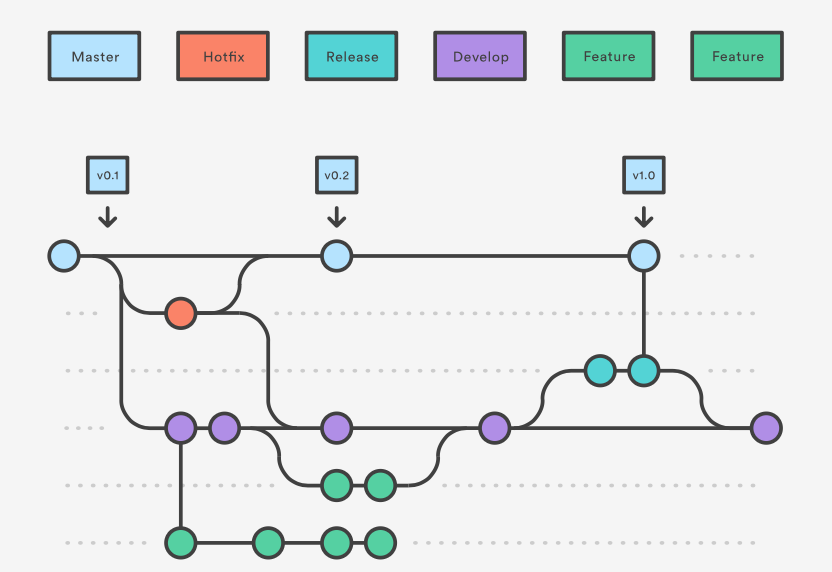
\includegraphics[width=0.8\textwidth]{images/GitFlow.png}
    \caption{Gitflow diagram, showing how branches should be created and named.}
    \label{Gitflow}
\end{figure}

\subsection{Git and GitHub within the application}
As software developers ourselves, we have used GitHub.
However, some Product Owners will have very limited or no experience at all with Git or GitHub.
We thought if the issues could be made directly by the Product Owner, it would make it easier for the developers to focus on working on the issues instead of creating and managing issues. 
This is where our product comes to the rescue.
It allows any Product Owner with no Git or GitHub experience, to create issues and tasks for developers to use.

Our application also allows the Product Owner to see communication between developers, and intervene and make sure that the developers are on track.

And since the application is already integrated with GitHub it was easy to implement a way for the Product Owner to be updated on the progress without the developers having to actively do so.
This is done by having the developer update the labels on the issue on GitHub, and the results in the application showing the status of the different issues. 

In this project we only implemented GitHub, since it is something we are very familiar with, but any alternative to GitHub such as BitBucket, Phabricator, GitLab, Atlassian, SourceForge or Launchpad would work just as well. However, they each would require specific implementation to be supported.
Such an implementation would likely be trivial and not require a lot of implementation, but for our MVP GitHub is enough as a prof of concept.
